\section{Modulul de rapoarte și decizii}

	O dată ce a fost implementat modulul de vânzări săptămânale, într-o stare incipientă (după cum s-a explicat în secțiunea anterioară), s-a trecut la dezvoltarea modulului de decizii.

	A fost conceput să se lege obligatoriu de o cerere de despăgubire și de o vânzare.

	Inițial, s-au construit rapoarte în format „.csv” (valori delimitate prin virgule).
	Ulterior s-a adăugat opțiunea de a putea vedea într-un tabel, în josul paginii, a rezultatelor rapoartelor, precum în figura~\ref{fig:statistics}.

	\begin{figure}
		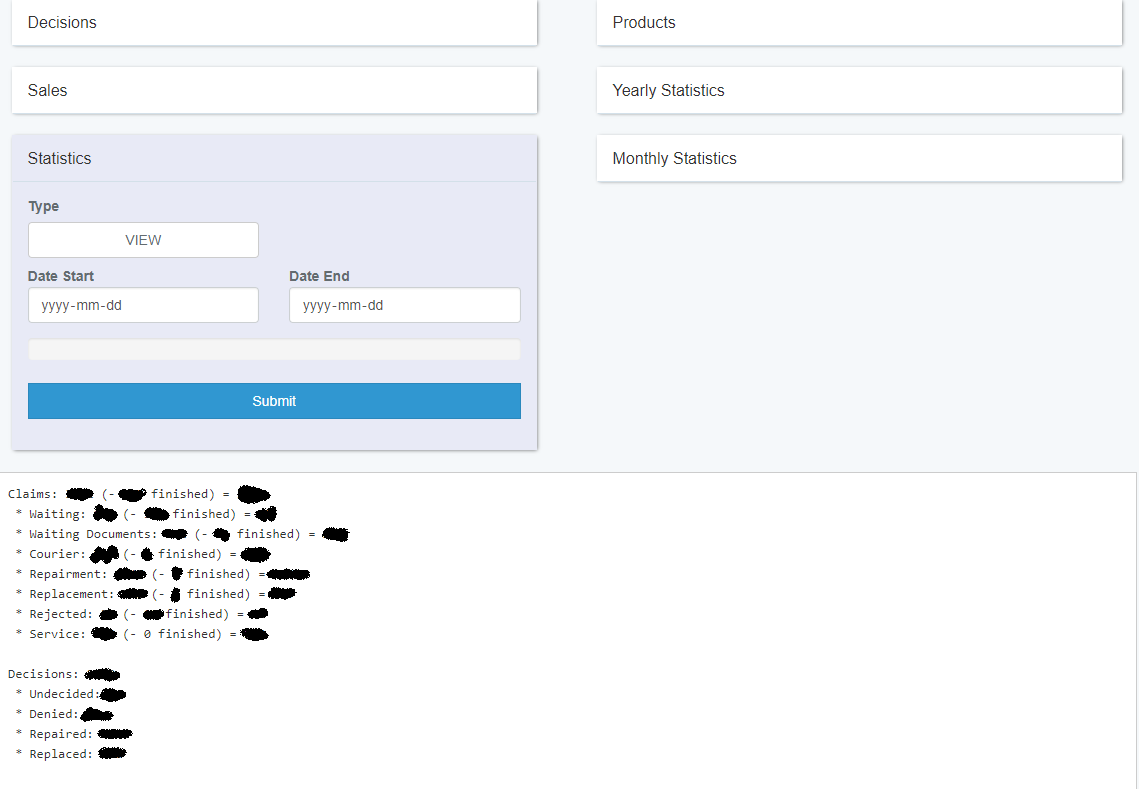
\includegraphics[width=\linewidth]{../imagini/statistics.png}
		\caption{Statistici}
		\label{fig:statistics}
	\end{figure}


	Gândirea pentru legătura dintre o vânzare și o decizie se învârte în jurul imposibilității existenței unei cereri de despăgubire, fără a fi fost vândut, al unui produs.

	Avantajul acestei abordări era ușurința aflării deciziilor multiple.
	Se putea afla ușor pentru că era aceeași vânzare, dar avea cereri multiple legate.

	În această perioadă de timp s-au mai adăugat și culori pentru starea curentă a unei cereri de despăgubiri, după cum se poate observa în figura~\ref{fig:color_coding}.

	\begin{figure}
		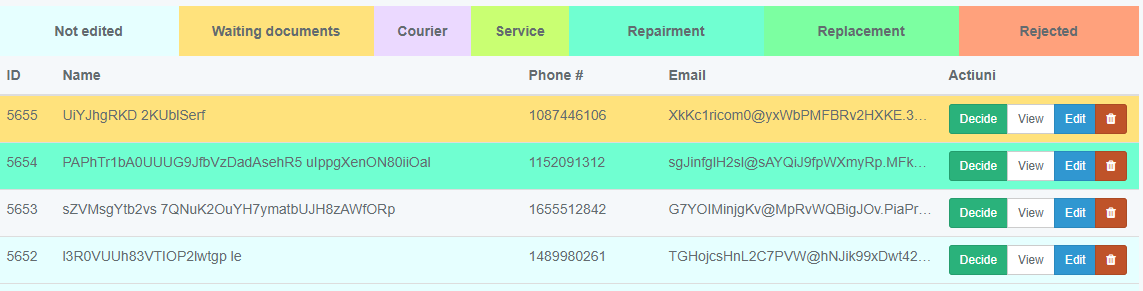
\includegraphics[width=\linewidth]{../imagini/color_coding.png}
		\caption{Culori cereri despăgubire}
		\label{fig:color_coding}
	\end{figure}

	După ce s-a terminat modulul de rapoarte, s-a revenit asupra modului de decizii pentru repararea micilor probleme numerice.
	Nu înțelesesem cum funcționează franciza, sau a sumei totale de plată.

	În acest moment s-a lucrat la adăugarea unei verificări a IMEI-ului clienților ce salvau o cerere de despăgubire de a limita depunerea unei cereri la un interval de 24 de ore pentru același IMEI.
	O problemă des întâlnită de operatorii aplicației erau cererile multiple de la aceeași persoană, cu puține modificări între ele.
	Prin limita de 24 de ore pentru același IMEI se împiedicau abuzurile.
	A fost scrisă astfel încât să nu se afle mai multe informații decât necesare.
